\chapter{Control of the ACTS}
\label{chap:control}
\input{sections/ForceControl-SpecialCases}

\section{Extension to the Complete ACTS Architecture}
\label{sec:highlevelarchitecture}
At high level, the architecture that enables the system to reach the goal is shown in Figure \ref{fig:control-high-level}.
\begin{figure}[h]
    \centering
    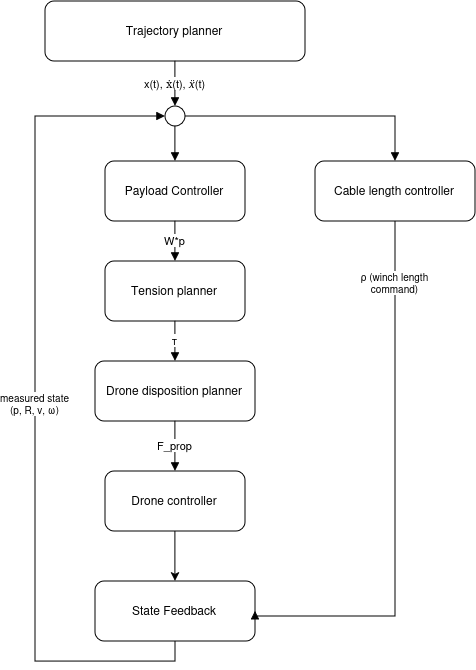
\includegraphics[width=0.6\linewidth]{images/diagrams/control_scheme.png}
    \caption{High level control scheme}
    \label{fig:control-high-level}
\end{figure}

\subsubsection{Trajectory planner}
The trajectory planner is able to compute the payload trajectory $x(t)$ and its velocity $\dot{x}(t)$ and acceleration $\ddot{x}(t)$ given the system's goal, such as:
\begin{enumerate}
    \item Make the payload fly;
    \item Bring the payload at the right height and orientation;
    \item Approach the façade.
\end{enumerate}
And/or the initial and final position of the payload.

\subsubsection{Payload Controller}
Then, the desired payload wrench $W_p^*$ is computed for each point in the trajectory based on the previous state of the system. 
The desired payload wrench is computed from a geometric PD controller. The translational component is given by

\begin{equation}
F_p^* = m_p g + K_p(p^*-p)+K_d(\dot p^*-\dot p),
\end{equation}
where \(p^*\) and \(p\) are the desired and current payload positions, respectively. For the rotational dynamics, the controller follows the geometric formulation on \(SE(3)\) \cite{lee_geometric_2010}. The attitude error and angular velocity error are defined as
\begin{equation}
    \begin{aligned}
e_R &=\frac{1}{2}\left(R^*^TR-R^TR^*\right)^\vee \\
e_\Omega &=\Omega-R^TR^*\Omega_d.
\end{aligned}
\end{equation} 
Where \((\cdot)^\vee\) denotes the inverse of the skew-symmetric (hat) operator. Since the controller performs set point regulation, the desired angular velocity is zero: \(\Omega_d=\mathbf{0}\), yielding $e_\Omega=\Omega$. The desired control moment in the world frame is then
\begin{equation}
    M_p^*=R(-K_Re_R - K_\Omega e_\Omega)
\end{equation}
and the desired payload wrench becomes
\begin{equation}
    W_p^*=
    \begin{bmatrix}
        F_p^*\\
        M_p^*
    \end{bmatrix}.
\end{equation}

\subsubsection{Winch-Level Cable Length Controller}
When transitioning the payload to a target pose along the planned trajectory, operational priority is given to the ground actuators due to their significantly higher mechanical stiffness and positioning precision compared to UAVs.

The ground subsystem is modeled as a 6-DOF Gough-Stewart parallel mechanism where the six ground cables act as active legs. Given the target payload position $p^*$ and target orientation matrix $R^*$, the ideal length $\rho_i^*$ for the $i$-th ground cable is defined geometrically by:
\begin{equation}
    \rho_i^* = \| a_i - (p^* + R^* \,^p b_i) \|
\end{equation}

 \begin{figure}
     \centering
     \includegraphics[width=0.5\linewidth]{images/StewartPlatform.png}
     \caption{Gogh Stewart schematics \cite{wang_adaptive_2023}}
     \label{fig:stewartplatform}
 \end{figure}

To account for the finite velocity of the winch motors, the desired cable length is not applied instantaneously. Instead, the cable-length reference is updated incrementally at each control step according to

\begin{equation}
    \rho_i(t+\Delta t)=\rho_i(t)+\Delta\rho_i,
\end{equation}

where the increment $\Delta\rho_i$ is limited such that $|\Delta\rho_i| = v_{\max}\Delta t$, with $v_{\max}$ being the maximum winch speed. The resulting cable-length reference is then sent to the actuator position controller. Consequently, the commanded cable length converges toward the desired value while respecting the physical velocity limits of the winch motors and avoiding unrealistically fast spool motions.

\subsubsection{Tension planner}
The tension planner is the layer responsible for guaranteeing that every cable stays taut throughout the motion. In fact, when working with ACTS, a payload wrench configuration is statically admissible if and only if there exists a set of strictly positive cable tensions ($\tau_i \ge \tau_{min} > 0$) that balance the target operational wrench. This is due to the fact that cables can only pull and not push. Mathematically, this layout optimization is formulated as:

 \begin{equation}
    \begin{aligned}
    \min_{p_a} \quad & \sum_{i=1}^{n_a}\|F_{prop}(p_{a, i}, \tau_{optimal, i})\|^2 + K \|J_p \tau_{optimal} -W_p^*\|^2\\
    \text{subj. to} \quad
    & x_i^2 + y_i^2 + z_i^2 = l_i^2 \quad \forall i \in [1, n_a]\\
    & \rho_{WCC}(\mathcal{U})\le 0\\
    & \rho_{IFC}(\mathcal{U})\le 0
    \end{aligned}
\end{equation} 

Which is a Nonlinear optimization Problem (NLP) due to the Euclidean distance constraints. % In Section \ref{sec:NLPtoQP}, we propose some ways to turn it into a Quadratic Programming problem (QP).

This objective function aims to minimize the propulsion force of the drones while satisfying the wrench equilibrium equations on the payload. The parameter $K$ acts as a penalty weight that prioritizes the tracking performance over energy efficiency; setting a high value (e.g., $K=100$), heavily penalizes any mismatch between the generated wrench and the commanded target wrench $W_p^*$.

For whatever positions $p_a$, the cable tensions $\tau$ are determined by a second inner loop
\begin{equation}
    \begin{aligned}
    \tau_{optimal} = \text{arg} \min_\tau & \, \frac{1}{2}\tau^\top H \tau \\
    \text{subj. to} \quad 
        & J_p^\top(\mathbf{u}) \tau = W_p^* \\
        & \tau_{min, i} \le \tau_i \le \tau_{max, i} \quad \forall i \in [1, n_a+ n_g]
    \end{aligned}
    \label{eq:tension-planner}
\end{equation}
The lower bound $\tau_{min, i}>0$ in the wrench feasible condition is what enforces the taut-cable requirement.

As the winch-level control drives $\mathbf{\rho} \to \mathbf{\rho}^*$, tracking the payload's motion toward its target pose, and $\mathbf{u} \to \mathbf{u}^*$, the achievable wrench set used by the tension planner is itself changing over the trajectory, since it depends on $\mathbf{u}$. As a consequence, $\mathbf{W}_p^*$ may be reachable at the target configuration but momentarily unreachable at the actual configuration, with all tensions kept strictly positive. When this occurs, Equation \ref{eq:tension-planner} should relax the equality constraint $\mathbf{J}_p^\top(\mathbf{u})\,\mathbf{\tau} = \mathbf{W}_p^*$ to a least-squares objective, while keeping $\tau_{min,i} > 0$ as a hard constraint. 

\begin{equation}
        \begin{aligned}
    \tau_{optimal} = \text{arg} \min_\tau & \, \left(\frac{1}{2}\tau^\top H \tau +\gamma \| J_p^\top (\mathbf{u}) \tau - W_p^*\|^2\right) \\
    \text{subj. to} \quad 
        & \tau_{min, i} \le \tau_i \le t_{max, i} \quad \forall i \in [1, n_a+ n_g]
    \end{aligned}
    \label{eq:tension-planner-relax}
\end{equation}


This guarantees that the tension planner always returns a taut solution, one that approximates the desired wrench as closely as the actual geometry allows, rather than returning no solution at all during the transient.

For the initial stage of development, this general QP is replaced by a simplified strategy: every cable tension is fixed at the minimum admissible value,
\begin{equation}
    \lVert \mathbf{\tau}_i^* \rVert = \tau_{min}, \qquad \forall i \in [1, n_a + n_g].
    \label{eq:tau-min-simplification}
\end{equation}



\subsubsection{Drone disposition planner}
Once the tension planner computes the scalar target tension magnitudes, the drones must dynamically adjust their orientation and propeller thrusts to impose these forces. 

From the static equilibrium balance (Equation \ref{eq:uavbalance}) the required propeller thrust vector is given by:

\begin{equation}
    \mathbf{F}_{prop,i} = \mathbf{F}_{a,i} - \mathbf{F}_{g,i} = \mathbf{J}_{a,i}^\top \tau_i + m_i \mathbf{g} = T_i \,^0_i\mathbf{R}\,\mathbf{e}_3, \qquad T_i = \lVert \mathbf{F}_{prop,i} \rVert
    \label{eq:drone-disposition}
\end{equation}
which is then handed to the attitude controller, responsible for aligning the body $z$-axis with the commanded thrust vector.

% \subsection{Quadratic Approximation of the UAV Disposition Problem}
% \label{sec:NLPtoQP}
% The nonlinear optimization problem presented in the previous section:
% $$
%     \begin{aligned}
%         \min_{p_a} \quad & \sum_{i=1}^{n_a}\|F_{prop}(p_{a, i}, \tau_{optimal})\|\\
%         \text{subj. to} \quad 
%         & x_i^2 + y_i^2 + z_i^2 = l_i^2 \quad \forall i \in [1, n_a]\\
%         & \rho_{WCC}(\mathcal{U})\le 0\\
%         & \rho_{IFC}(\mathcal{U})\le 0
%     \end{aligned}
% $$
% can be rewritten as a quadratic problem where possible.

% \subsubsection{Wrench closure condition}
% The rank condition $\text{rank}(J_p) = 6$ is not a smooth inequality. To overcome this problem, we could: 

% \begin{itemize}
%     \item Use the manipulability index squared $w^2=\det(J_p J_p^\top)\ge w_{\text{min}}^2>0$ in which $w=0$ indicates a singular configuration;
%     \item Impose positive value for the smaller singular value $\epsilon$: $\sigma_{\text{min}}(J_p) \ge \epsilon$
% \end{itemize}


% \subsubsection{The cost function}
% The objective function can be approximated by replacing the sum of Euclidean norms with the sum of squared Euclidean norms,

% \begin{equation}
%     \min_{p_a}\sum_{i=1}^{n_a}\|F_{prop}(p_{a, i}, \tau_{optimal})\| \approx \min_{p_a}\sum_{i=1}^{n_a}\|F_{prop}(p_{a, i}, \tau_{optimal})\|_2 = \min_{p_a}\sum_{i=1}^{n_a}F_{prop}^\top F_{prop}
% \end{equation}
% as for definition $\|u\|_2 = \sqrt{u^\top u}$. This approximation penalizes large outliners more than small ones.

% Therefore, the problem becomes:

% \begin{equation}
%       \begin{aligned}
%         \min_{p_a} \quad & \sum_{i=1}^{n_a}F_{prop}^\top F_{prop}\\
%         \text{subj. to} \quad 
%         & x_i^2 + y_i^2 + z_i^2 = l_i^2 \quad \forall i \in [1, n_a]\\
%         & w_{\text{min}}^2 - w^2 \le 0\\
%         & d_{\text{safe}} - d_{ij} \le 0 \\
%         & d_{\text{safe}} - d_{i} \le 0 \\
%     \end{aligned}
% \end{equation}